%%%%%%%%%% NO OLVIDAR COLOCAR ESTE COMENTARIO CON EL NUMERO DE EJERCICIO %%%%%%%%%%%%%
%%%%%%%%%%%%%%%%%%% EJERCICIO 1 %%%%%%
\textbf{Ejemplo 1. Selección entre dos motores}\newline
Se necesita adquirir un motor para la planta de acabados de una fábrica. Las dos alternativas cumplen las especificaciones técnicas. La información económica es la siguiente:
\begin{center}
	\renewcommand{\arraystretch}{1.3}
	\begin{tabular}{|l|c|c|}
		\hline
		\rowcolor[HTML]{FFB183}
		\textbf{Concepto} & \textbf{Alternativa A} & \textbf{Alternativa B} \\ \hline
		Costo inicial ($P$) & COP 100.000 & COP 500.000 \\ \hline
		Costo de operación mensual ($R_m$) & COP 5.000 & COP 10.000 \\ \hline
		Vida útil ($n$) & 5 años & 20 años \\ \hline
		Valor de salvamento ($VS$) & COP 15.000 & COP 150.000 \\ \hline
		Reparación general en el año 12 & --- & COP 200.000 \\ \hline
	\end{tabular}
\end{center}

Tasa: 2,5\% nominal anual mes vencido (namv). Se pide determinar la mejor alternativa mediante el CAUE.\\

\textbf{Solución.}\\

\begin{center}
	\renewcommand{\arraystretch}{1.5}% Margenes de las celdas
	\small% Tamaño de letra de la tabla para que quepan las expresiones con COP
	\begin{longtable}[H]{|c|c|c|}
		\hline
		\rowcolor[HTML]{FFB183}
		%%%%% INICIO ASIGNACIÓN FECHA FOCAL %%%%%%%
		\multicolumn{3}{|c|}{\cellcolor[HTML]{FFB183}\textbf{1. Asignación período focal}} \\ \hline
		\multicolumn{3}{|c|}{$pf = 0\text{ pav (inicio de la evaluación)}$} \\ \hline
		
		%%%%% INICIO DECLARACIÓN DE VARIABLES %%%%%%%
		\rowcolor[HTML]{FFB183}
		\multicolumn{3}{|c|}{\cellcolor[HTML]{FFB183}\textbf{2. Declaración de variables}} \\ \hline
		\cellcolor[HTML]{FFB183}\textbf{Valores monetarios} & 
		\cellcolor[HTML]{FFB183}\textbf{Valores no monetarios} &
		\cellcolor[HTML]{FFB183}\textbf{Incógnitas} \\ \hline
		
		$P_A = \text{COP } 100.000$ & $j = 2{,}5\%\text{ namv} ; m = 12$ & $CAUE_A = \text{? COP/año}$ \\
		$VS_A = \text{COP } 15.000$ & $i_m = 0{,}208333\%\text{ pmv}$ & $CAUE_B = \text{? COP/año}$ \\
		$R_{mA} = \text{COP } 5.000/\text{mes}$ & $i_{\text{año}} = 2{,}528846\%\text{ pav}$ & \\
		$P_B = \text{COP } 500.000$ & $n_A = 5\text{ pav}$ & \\
		$VS_B = \text{COP } 150.000$ & $n_B = 20\text{ pav}$ & \\
		$R_{mB} = \text{COP } 10.000/\text{mes}$ & & \\
		$C_{\text{rep},B} = \text{COP } 200.000\text{ en } t = 12$ & & \\ \hline

		%%%%% INICIO FLUJO DE CAJA
		\rowcolor[HTML]{FFB183}
		\multicolumn{3}{|c|}{\cellcolor[HTML]{FFB183}\textbf{3. Diagrama de flujo de caja}} \\ \hline
		
		\multicolumn{3}{|c|}{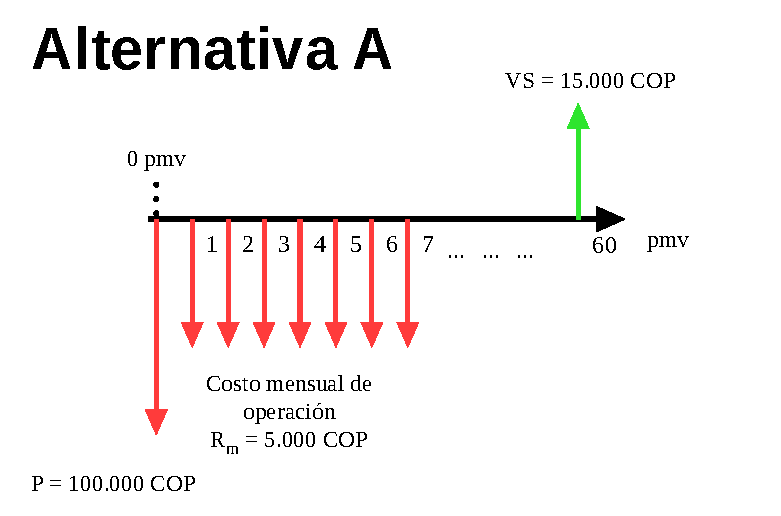
\includegraphics[trim=-5 -5 -5 -5, width=12cm, keepaspectratio]{10_Capitulo/img/ejemplos/PDFs/1/Ejemplo_1_A.pdf}}\\ \hline
		\multicolumn{3}{|c|}{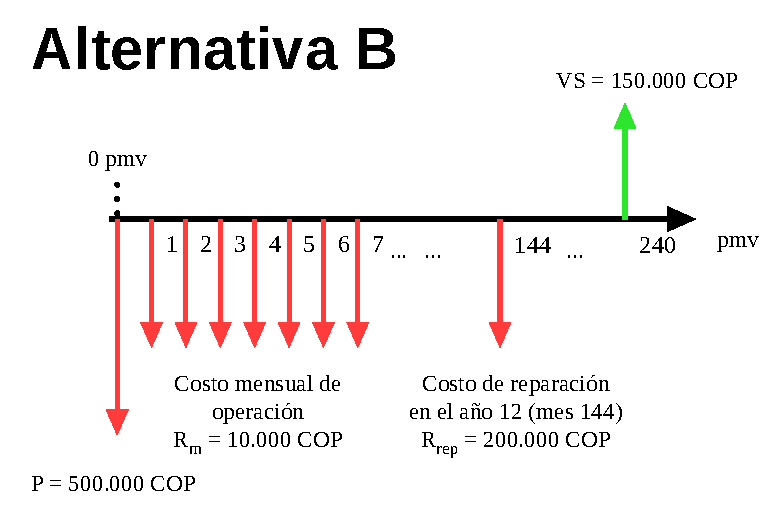
\includegraphics[trim=-5 -5 -5 -5, width=12cm, keepaspectratio]{10_Capitulo/img/ejemplos/PDFs/1/Ejemplo_1_B.pdf}}\\ \hline
		\multicolumn{3}{|p{14cm}|}{\small Los costos mensuales de operación se agrupan y acumulan al final de cada año; por eso el diagrama anual utiliza $i_{\text{año}}$ y períodos pav. La reparación de B ocurre al final del año 12.} \\ \hline

		%%%%% INICIO DECLARACIÓN FORMULAS
		\rowcolor[HTML]{FFB183}
		\multicolumn{3}{|c|}{\cellcolor[HTML]{FFB183}\textbf{4. Declaración de fórmulas}} \\ \hline

		\multicolumn{3}{|c|}{$i_m = \dfrac{j}{12} \quad ; \quad i_{\text{año}} = (1+i_m)^{12} - 1$}\\ 
		\multicolumn{3}{|c|}{$F_{op,\text{año}} = R_m \left[ \dfrac{(1+i_m)^{12}-1}{i_m} \right] \quad (F/A)$}\\
		\multicolumn{3}{|c|}{$A_P = P \left[ \dfrac{i(1+i)^n}{(1+i)^n-1} \right] \quad (A/P) \quad ; \quad A_F = F \left[ \dfrac{i}{(1+i)^n-1} \right] \quad (A/F)$}\\
		\multicolumn{3}{|c|}{$VP_{\text{rep}} = C_{\text{rep}}(1+i)^{-12} \quad ; \quad A_{\text{rep}} = VP_{\text{rep}} (A/P, i, 20)$}\\
		\multicolumn{3}{|c|}{$CAUE = \sum \text{Ingresos}_{\text{anualizados}} - \sum \text{Egresos}_{\text{anualizados}}$}\\
		\hline

		%%%%%% INICIO DESARROLLO MATEMÁTICO
		\rowcolor[HTML]{FFB183}
		\multicolumn{3}{|c|}{\cellcolor[HTML]{FFB183}\textbf{5. Desarrollo matemático}} \\ \hline

		\multicolumn{3}{|l|}{\textbf{Conversión de tasa:}} \\
		\multicolumn{3}{|l|}{$i_m = \dfrac{0{,}025}{12} = 0{,}002083333 = 0{,}208333\%\text{ pmv}$} \\
		\multicolumn{3}{|l|}{$i_{\text{año}} = (1 + 0{,}002083333)^{12} - 1 = 0{,}025288457 = 2{,}528846\%\text{ pav}$} \\ \hline

		\multicolumn{3}{|l|}{\textbf{Valor anual acumulado de los costos mensuales de operación:}} \\
		\multicolumn{3}{|l|}{Alternativa A: $F_{op,A} = 5.000 \cdot \dfrac{(1 + 0{,}002083333)^{12} - 1}{0{,}002083333} = \text{COP } 60.692{,}30/\text{año}$} \\
		\multicolumn{3}{|l|}{Alternativa B: $F_{op,B} = 10.000 \cdot \dfrac{(1 + 0{,}002083333)^{12} - 1}{0{,}002083333} = \text{COP } 121.384{,}59/\text{año}$} \\ \hline

		\cellcolor[HTML]{FFB183}\textbf{Componente anual equivalente} & \cellcolor[HTML]{FFB183}\textbf{Alternativa A (COP/año)} & \cellcolor[HTML]{FFB183}\textbf{Alternativa B (COP/año)} \\ \hline
		Recuperación de inversión inicial & $100.000(A/P, 2{,}528846\%, 5) = 21.542{,}56$ & $500.000(A/P, 2{,}528846\%, 20) = 32.161{,}02$ \\ \hline
		Costo mensual acumulado al cierre & $60.692{,}30$ & $121.384{,}59$ \\ \hline
		Reparación del año 12 & --- & $200.000(1{,}025288457)^{-12}(A/P, 2{,}528846\%, 20) = 9.533{,}16$ \\ \hline
		Crédito por salvamento & $15.000(A/F, 2{,}528846\%, 5) = 2.852{,}06$ & $150.000(A/F, 2{,}528846\%, 20) = 5.855{,}04$ \\ \hline

		\multicolumn{3}{|l|}{\textbf{CAUE de cada alternativa:}} \\
		\multicolumn{3}{|l|}{$CAUE_A = +2.852{,}06 - 21.542{,}56 - 60.692{,}30 = -\text{COP } 79.382{,}80/\text{año}$} \\
		\multicolumn{3}{|l|}{$CAUE_B = +5.855{,}04 - 32.161{,}02 - 9.533{,}16 - 121.384{,}59 = -\text{COP } 157.223{,}74/\text{año}$} \\ \hline

		%%%%%% INICIO RESPUESTA
		\rowcolor[HTML]{FFB183}
		\multicolumn{3}{|c|}{\cellcolor[HTML]{FFB183}\textbf{6. Respuesta}} \\ \hline

		\multicolumn{3}{|c|}{\parbox{14cm}{\centering\strut Se selecciona la alternativa A. Su CAUE es menos negativo y representa un costo anual equivalente menor: COP 79.382,80/año, frente a COP 157.223,74/año de la alternativa B.\strut}} \\ \hline
	\end{longtable}
\end{center}
%%%%%%%%%%%%%%%%%%%%%%%%%%FIN EJERCICIO 1 %%%%%%%%%%%%%%%%%%%%%%%%%%%
